% Generated by thesis/ch7/exp1/networks.py -- do not edit by hand.
\ifdefined\netfigheight\else\newlength{\netfigheight}\setlength{\netfigheight}{0.9\textwidth}\fi
\begin{sidewaysfigure}
  \centering
  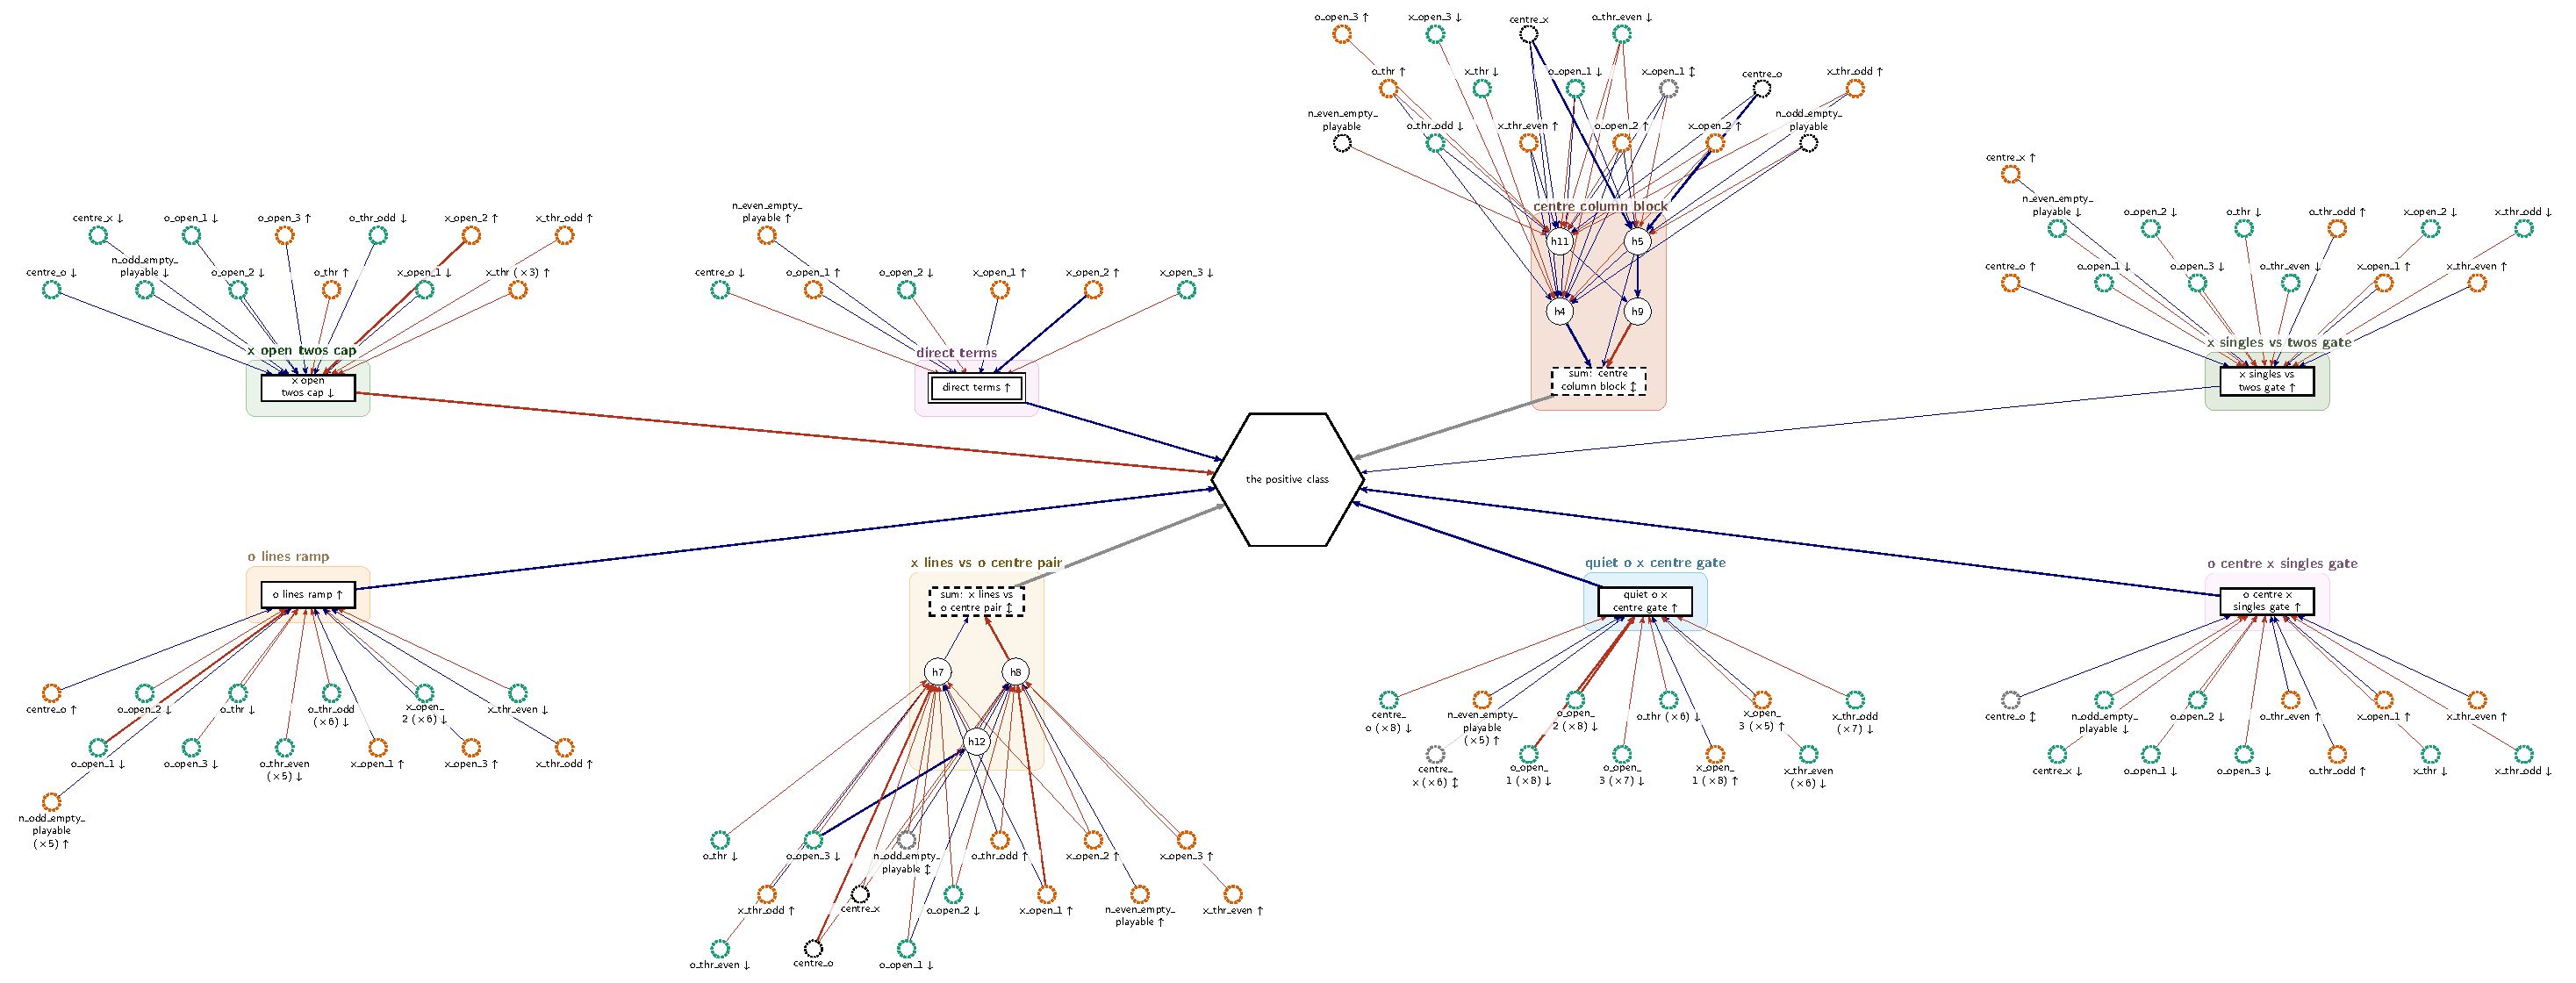
\includegraphics[width=\textheight,height=\netfigheight,keepaspectratio]{figures/exp1/networks/c4lf-lines-heavy-s0-explained}
  \caption{Connect-4, lines, seed 0: the explained network, each top-level part collapsed into one box (its output), the inputs each part reads below it. Grey edges: the inputs a collapsed part reads (no single weight); a part reading many input columns has them drawn as one input. Arrows on inputs and boxes: the direction of the effect on the final prediction (up raises it, down lowers it, double arrow depends). Edges: blue, a positive weight (raises the score); red, a negative weight (lowers it); thicker, a larger weight.}
  \label{fig:exp1-net-c4lf-lines-heavy-s0-explained}
\end{sidewaysfigure}
